\documentclass[border=6pt]{standalone}
\usepackage{tikz}
\begin{document}
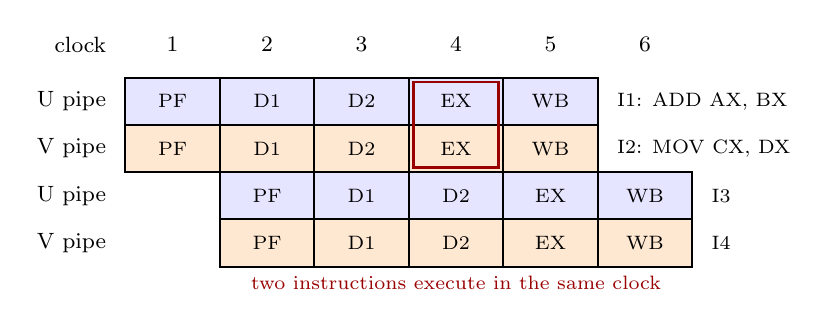
\begin{tikzpicture}[font=\small,x=1.2cm,y=0.6cm,
 st/.style={draw,thick,minimum width=1.2cm,minimum height=0.6cm,inner sep=0,font=\scriptsize}]
\foreach \c in {1,...,6} \node[font=\footnotesize] at (\c-0.5,1.2) {\c};
\node[anchor=east,font=\footnotesize] at (-0.1,1.2) {clock};
\foreach \r/\p/\s/\l/\c in {0/U/0/{I1: ADD AX, BX}/blue!10,1/V/0/{I2: MOV CX, DX}/orange!18,2/U/1/{I3}/blue!10,3/V/1/{I4}/orange!18} {
  \node[anchor=east,font=\footnotesize] at (-0.1,-\r) {\p\ pipe};
  \foreach \k/\n in {0/PF,1/D1,2/D2,3/EX,4/WB} \node[st,fill=\c] at (\s+\k+0.5,-\r) {\n};
  \node[anchor=west,font=\scriptsize] at (\s+5.1,-\r) {\l};
}
\draw[thick,red!60!black] (3.05,0.4) rectangle (3.95,-1.4);
\node[font=\scriptsize,red!60!black,anchor=north] at (3.5,-3.5) {two instructions execute in the same clock};
\end{tikzpicture}
\end{document}
